% Source PDF page 403 (printed p. 389)
\begin{figure}[htbp]\centering
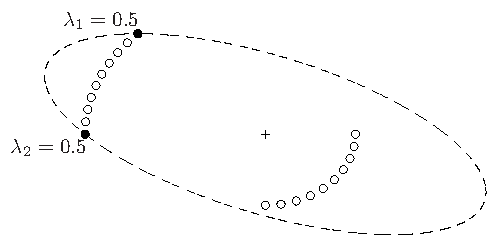
\includegraphics[width=.68\textwidth]{figures/ch07-figure-9.pdf}
\caption*{图7.9\quad 实验设计例子。20个候选测量向量以圆圈表示。D最优设计使用两个实心圆所示的测量向量，并各赋予相同权重 $\lambda_i=0.5$。椭球是包含各点 $v_i$、以原点为中心的最小体积椭球。}
\end{figure}
\begin{figure}[htbp]\centering
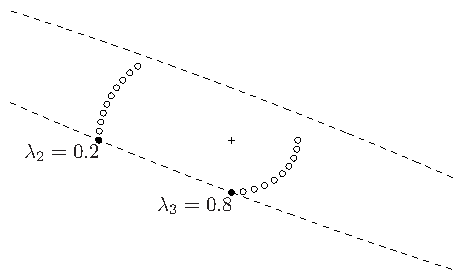
\includegraphics[width=.68\textwidth]{figures/ch07-figure-10.pdf}
\caption*{图7.10\quad E最优设计使用两个测量向量。虚线为椭球 $\{x\mid x^{\T}W^\star x\le1\}$ 的部分边界，其中 $W^\star$ 是对偶问题（7.30）的解。}
\end{figure}
\begin{figure}[htbp]\centering
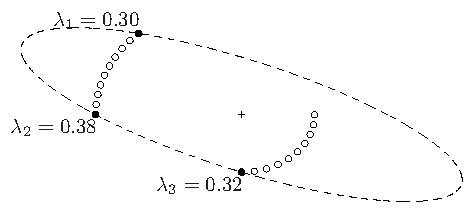
\includegraphics[width=.68\textwidth]{figures/ch07-figure-11.pdf}
\caption*{图7.11\quad A最优设计使用三个测量向量。虚线为对偶问题（7.31）的解所对应的椭球 $\{x\mid x^{\T}W^\star x\le1\}$。}
\end{figure}

% Source PDF page 404 (printed p. 390)
\begin{figure}[htbp]\centering
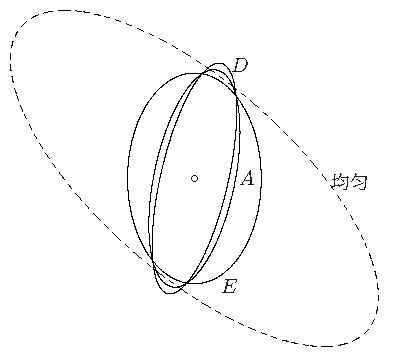
\includegraphics[width=.70\textwidth]{figures/ch07-figure-12.pdf}
\caption*{图7.12\quad D最优、A最优、E最优和均匀设计的90\%置信椭球形状。}
\end{figure}

\subsection{扩展}
\subsubsection*{资源限制}
假设每类实验有相应代价 $c_i$，它可以表示用 $v_i$ 进行一次实验的经济成本或所需时间。总成本，或实验顺序执行时的总时间，为
\[
 m_1c_1+\cdots+m_pc_p=mc^{\T}\lambda.
\]
可在基本实验设计问题中加入线性不等式 $mc^{\T}\lambda\le B$，其中 $B$ 为预算，以限制总成本。也可以加入多个线性不等式，表示多项资源的限制。

\subsubsection*{每次实验进行多个测量}
还可以推广到每次实验产生多个测量的情形。换言之，选择某个可能实验并执行后，会获得若干测量。可沿用前面的记号，将 $v_i$ 取为 $\R^{n\times k_i}$ 中的矩阵：
\[
 v_i=\begin{bmatrix}u_{i1}&\cdots&u_{ik_i}\end{bmatrix},
\]
其中 $k_i$ 是执行实验 $v_i$ 后得到的标量测量个数。在这种更复杂的设定下，误差协方差矩阵的形式完全不变。

结合表示成本或时间限制的附加线性不等式，可以描述同时进行一组测量带来的成本优惠或时间节省。例如，假设同时进行标量测量 $v_1,v_2$ 的成本，低于分别进行两次测量的成本之和。

% Source PDF page 405 (printed p. 391)
令 $v_3$ 为矩阵
\[
 v_3=\begin{bmatrix}v_1&v_2\end{bmatrix},
\]
并用 $c_1,c_2,c_3$ 分别表示单独进行第一个测量、单独进行第二个测量，以及同时进行两者的成本。

求解实验设计问题后，$\lambda_1$ 给出应单独进行第一个实验的次数比例，$\lambda_2$ 给出单独进行第二个实验的比例，$\lambda_3$ 给出同时进行两个实验的比例。通常会预期这几类中有所取舍，不会同时出现 $\lambda_1>0$、$\lambda_2>0$、$\lambda_3>0$。

% Source PDF page 406 (printed p. 392)
\section*{文献说明}
\addcontentsline{toc}{section}{文献说明}
ML和MAP估计、假设检验与检测，可参阅统计学、模式识别、统计信号处理或通信方面的书籍，例如 Bickel 和 Doksum [BD77]，Duda、Hart 和 Stork [DHS99]，Scharf [Sch91]，或 Proakis [Pro01]。

Logistic回归见 Hastie、Tibshirani 和 Friedman [HTF01，第4.4节]。第355页的协方差估计问题见 Anderson [And70]。

20世纪60年代，Isii [Isi64]、Marshall 和 Olkin [MO60]、Karlin 和 Studden [KS66，第12章] 等对Chebyshev不等式的推广进行了广泛研究。较近，Bertsimas 和 Sethuraman [BS00]、Lasserre [Las02] 建立了其与半正定规划的联系。

第7.5节中的A、D、E最优性是最优实验设计文献中的标准术语，例如 Pukelsheim [Puk93]。D最优设计对偶问题的几何解释见 Titterington [Tit75]。

% Source PDF page 407 (printed p. 393)
\section*{习题}
\addcontentsline{toc}{section}{习题}
\subsection*{估计}
\paragraph{7.1}
\textbf{指数分布噪声下的线性测量。}说明噪声服从指数分布时，如何求解ML估计问题（7.2），其密度为
\[
 p(z)=\begin{cases}(1/a)e^{-z/a}&z\ge0,\\0&z<0,\end{cases}
\]
其中 $a>0$。

\paragraph{7.2}
\textbf{ML估计与 $\ell_\infty$ 范数逼近。}考虑第352页的线性测量模型 $y=Ax+v$，噪声均匀分布，密度为
\[
 p(z)=\begin{cases}1/(2\alpha)&\abs z\le\alpha,\\0&\abs z>\alpha.\end{cases}
\]
如第352页例7.1所述，任意满足 $\norm{Ax-y}_\infty\le\alpha$ 的 $x$ 都是ML估计。

现设参数 $\alpha$ 未知，需要将它与 $x$ 一起估计。证明：求解 $\ell_\infty$ 范数逼近问题
\[
 \text{最小化}\quad\norm{Ax-y}_\infty
\]
即可找到 $x,\alpha$ 的ML估计，其中 $a_i^{\T}$ 为 $A$ 的各行。

\paragraph{7.3}
\textbf{Probit模型。}设随机变量 $y\in\{0,1\}$ 由下式给出：
\[
 y=\begin{cases}1&a^{\T}u+b+v\le0,\\0&a^{\T}u+b+v>0,\end{cases}
\]
其中 $u\in\R^n$ 是解释变量向量，与第354页Logistic模型中的意义相同，$v$ 为零均值、单位方差的高斯变量。

给定数据对 $(u_i,y_i)$，$i=1,\ldots,N$，将估计 $a,b$ 的ML问题写成凸优化问题。

\paragraph{7.4}
\textbf{多元正态分布的协方差与均值估计。}考虑根据 $N$ 个独立样本 $y_1,y_2,\ldots,y_N\in\R^n$，估计高斯概率密度
\[
 p_{R,a}(y)=(2\pi)^{-n/2}\det(R)^{-1/2}
 \exp\bigl(-(y-a)^{\T}R^{-1}(y-a)/2\bigr)
\]
的协方差矩阵 $R$ 与均值 $a$。
\begin{enumerate}[label=(\alph*)]
\item 先考虑对 $R,a$ 没有附加约束的估计问题。令 $\mu,Y$ 为样本均值与协方差，定义为
\[
 \mu=\frac1N\sum_{k=1}^Ny_k,\qquad
 Y=\frac1N\sum_{k=1}^N(y_k-\mu)(y_k-\mu)^{\T}.
\]
证明对数似然函数
\[
 l(R,a)=-(Nn/2)\log(2\pi)-(N/2)\log\det R
 -(1/2)\sum_{k=1}^N(y_k-a)^{\T}R^{-1}(y_k-a)
\]

% Source PDF page 408 (printed p. 394)
可表示为
\[
 l(R,a)=\frac N2\bigl(-n\log(2\pi)-\log\det R
 -\tr(R^{-1}Y)-(a-\mu)^{\T}R^{-1}(a-\mu)\bigr).
\]
利用该表达式证明：若 $Y\succ0$，$R,a$ 的ML估计唯一，且为
\[
 a_{\mathrm{ml}}=\mu,\qquad R_{\mathrm{ml}}=Y.
\]
\item 对数似然函数包含凸项 $-\log\det R$，因此其凹性并不显然。证明：在区域
\[
 R\preceq2Y
\]
内，$l$ 关于 $R,a$ 联合凹。这意味着，只要约束包含 $R\preceq2Y$，即 $R$ 的估计不超过无约束ML估计的两倍，就可以在凸约束下，用凸优化同时计算 $R,a$ 的ML估计。
\end{enumerate}

\paragraph{7.5}
\textbf{Markov链估计。}考虑一个具有 $n$ 个状态的Markov链，转移概率矩阵 $P\in\R^{n\times n}$ 定义为
\[
 P_{ij}=\Prob(y(t+1)=i\mid y(t)=j).
\]
转移概率必须满足 $P_{ij}\ge0$、$\sum_{i=1}^nP_{ij}=1$，$j=1,\ldots,n$。考虑由观测样本序列 $y(1)=k_1$、$y(2)=k_2$、$\ldots$、$y(N)=k_n$ 估计转移概率。
\begin{enumerate}[label=(\alph*)]
\item 证明：若 $P_{ij}$ 无其他先验约束，其ML估计为经验转移频率：$\widehat P_{ij}$ 是观测样本中状态从 $j$ 转移到 $i$ 的次数，与状态为 $j$ 的次数之比。
\item 假设Markov链的一个平衡分布 $p$ 已知，即向量 $q\in\R_+^n$ 满足 $\one^{\T}q=1$、$Pq=q$。证明根据观测序列及已知 $q$ 求 $P$ 的ML估计，可以表示为凸优化问题。
\end{enumerate}

\paragraph{7.6}
\textbf{均值与方差估计。}考虑密度为 $p$ 的随机变量 $x\in\R$，它已标准化，即零均值、单位方差。对 $x$ 作仿射变换得到 $y=(x+b)/a$，其中 $a>0$。$y$ 的均值为 $b/a$，方差为 $1/a^2$。当 $a,b$ 分别在 $\R_+$、$\R$ 上变化时，通过缩放与平移 $p$，产生由均值和方差唯一参数化的一族密度。

证明：若 $p$ 对数凹，给定 $y$ 的样本 $y_1,\ldots,y_n$，求 $a,b$ 的ML估计是凸问题。

作为例子，假设 $p$ 是标准化的Laplace密度 $p(x)=e^{-2\abs x}$，求出 $a,b$ 的ML估计的解析解。

\paragraph{7.7}
\textbf{Poisson分布的ML估计。}设随机变量 $x_i$，$i=1,\ldots,n$，相互独立，服从Poisson分布
\[
 \Prob(x_i=k)=\frac{e^{-\mu_i}\mu_i^k}{k!},
\]
均值 $\mu_i$ 未知。$x_i$ 表示某段时间内 $n$ 类可能独立事件中，第 $i$ 类发生的次数。例如，在发射断层成像中，它们可以表示 $n$ 个源发射的光子数。

考虑一个用于确定均值 $\mu_i$ 的实验，其中有 $m$ 个检测器。若发生事件 $i$，则它以概率 $p_{ji}$ 被检测器 $j$ 检出。

% Source PDF page 409 (printed p. 395)
假设概率 $p_{ji}$ 已知，且 $p_{ji}\ge0$、$\sum_{j=1}^mp_{ji}\le1$。检测器 $j$ 记录的事件总数记为 $y_j$，
\[
 y_j=\sum_{i=1}^ny_{ji},\qquad j=1,\ldots,m.
\]
根据观测值 $y_j$，$j=1,\ldots,m$，将估计均值 $\mu_i$ 的ML问题写成凸优化问题。

\emph{提示：}变量 $y_{ji}$ 服从均值为 $p_{ji}\mu_i$ 的Poisson分布，即
\[
 \Prob(y_{ji}=k)=\frac{e^{-p_{ji}\mu_i}(p_{ji}\mu_i)^k}{k!}.
\]
均值分别为 $\lambda_1,\ldots,\lambda_n$ 的 $n$ 个独立Poisson变量之和，仍服从Poisson分布，均值为 $\lambda_1+\cdots+\lambda_n$。

\paragraph{7.8}
\textbf{利用符号测量的估计。}考虑测量模型
\[
 y_i=\operatorname{sign}(a_i^{\T}x+b_i+v_i),\qquad i=1,\ldots,m,
\]
其中 $x\in\R^n$ 为待估向量，$y_i\in\{-1,1\}$ 为测量值。向量 $a_i\in\R^n$、标量 $b_i\in\R$ 已知，$v_i$ 是独立同分布、具有对数凹概率密度的噪声。可假设 $a_i^{\T}x+b_i+v_i=0$ 不会发生。证明 $x$ 的最大似然估计是凸优化问题。

\paragraph{7.9}
\textbf{传感器非线性未知时的估计。}考虑测量模型
\[
 y_i=f(a_i^{\T}x+b_i+v_i),\qquad i=1,\ldots,m,
\]
其中 $x\in\R^n$ 为待估向量，$y_i\in\R$ 为测量值，$a_i\in\R^n$、$b_i\in\R$ 已知，$v_i$ 为独立同分布、密度对数凹的噪声。表示测量非线性的函数 $f:\R\to\R$ 未知，但已知它对所有 $t$ 满足 $f'(t)\in[l,u]$，其中 $0<l<u$ 已知。

说明如何用凸优化找到 $x$ 以及函数 $f$ 的最大似然估计。这是无限维ML估计问题，但可以采用非正式的处理和解释。

\paragraph{7.10}
\textbf{$\R^k$ 上的非参数分布。}考虑随机变量 $x\in\R^k$，取值于有限集 $\{\alpha_1,\ldots,\alpha_n\}$，分布为
\[
 p_i=\Prob(x=\alpha_i),\qquad i=1,\ldots,n.
\]
证明 $X$ 的协方差下界
\[
 S\preceq\E(X-\E X)(X-\E X)^{\T}
\]
是关于 $p$ 的凸约束。

\subsection*{最优检测器设计}
\paragraph{7.11}
\textbf{随机化检测器。}证明每个随机化检测器都能表示为一组确定性检测器的凸组合：若
\[
 T=\begin{bmatrix}t_1&t_2&\cdots&t_n\end{bmatrix}\in\R^{m\times n}
\]
满足 $t_k\succeq0$、$\one^{\T}t_k=1$，则可写为
\[
 T=\theta_1T_1+\cdots+\theta_NT_N,
\]

% Source PDF page 410 (printed p. 396)
其中 $T_i$ 是每列恰有一个元素为一的0--1矩阵，$\theta_i\ge0$、$\sum_{i=1}^N\theta_i=1$。最多可能需要多少个确定性检测器，即 $N$ 最大需要多大？

可作如下解释：随机化检测器能够由 $N$ 个确定性检测器组成的检测器组实现。观测到 $X=k$ 时，估计器从 $\{1,\ldots,N\}$ 中以概率 $\Prob(j=i)=\theta_i$ 选取随机索引，再使用确定性检测器 $T_j$。

\paragraph{7.12}
\textbf{最优行动。}检测器设计中，给定各列为概率分布的矩阵 $P\in\R^{n\times m}$，然后设计各列也为概率分布的矩阵 $T\in\R^{m\times n}$，使 $D=TP$ 的对角元大、非对角元小。本题研究对应的对偶问题：给定 $P$，寻找各列为概率分布的矩阵 $S\in\R^{m\times n}$，使 $\widetilde D=PS\in\R^{n\times n}$ 对角元大、非对角元小。具体取目标为最大化 $\widetilde D$ 的最小对角元。

可作如下解释：有 $n$ 种结果，其发生概率取决于采取 $m$ 种输入或行动中的哪一种；$P_{ij}$ 是采取行动 $j$ 时出现结果 $i$ 的概率。目标是寻找一种随机化策略，使任何指定结果尽可能发生。策略由矩阵 $S$ 给出：希望结果 $i$ 发生时，以概率 $S_{ji}$ 采取行动 $j$。矩阵 $\widetilde D$ 给出行动错误概率矩阵：$\widetilde D_{ij}$ 是希望结果 $j$ 发生时，实际出现结果 $i$ 的概率。特别地，$\widetilde D_{ii}$ 是希望结果 $i$ 发生时，结果 $i$ 实际发生的概率。

证明这个问题具有简单解析解。证明与相应检测器问题不同，这里总有确定性的最优解。

\emph{提示：}证明问题关于 $S$ 的各列可分。

\subsection*{Chebyshev界与Chernoff界}
\paragraph{7.13}
\textbf{有限集上的Chebyshev型不等式。}设随机变量 $X$ 取值于集合 $\{\alpha_1,\alpha_2,\ldots,\alpha_m\}$，$S$ 是 $\{\alpha_1,\ldots,\alpha_m\}$ 的子集。$X$ 的分布未知，但已知 $n$ 个函数 $f_i$ 的期望：
\begin{equation}
 \E f_i(X)=b_i,\qquad i=1,\ldots,n.\tag{7.32}
\end{equation}
证明线性规划
\[
\begin{array}{ll}
\text{最小化}&\displaystyle x_0+\sum_{i=1}^nb_ix_i\\
\text{满足}&\displaystyle x_0+\sum_{i=1}^nf_i(\alpha)x_i\ge1,\quad\alpha\in S,\\
&\displaystyle x_0+\sum_{i=1}^nf_i(\alpha)x_i\ge0,\quad\alpha\notin S,
\end{array}
\]
的最优值为 $\Prob(X\in S)$ 的上界，对所有满足（7.32）的分布都成立，变量为 $x_0,\ldots,x_n$。证明总存在某个分布取到该上界。
